\chapter{Biomass functions and nutrient contents of European beech, oak, sycamore maple and ash and their meaning for the biomass supply chain}
\label{chap:bm}
{\large Kai Husmann$^1$ - Sabine Rumpf$^2$ - J�rgen Nagel$^{2}$}\\

\vspace{3cm}
\noindent
$^1$Department of Forest Economics and Forest Management,\\ University of G�ttingen, B�sgenweg 3, 37077 G�ttingen, Germany \\

%\vspace{0.5cm}
\noindent
$^2$Northwest German Forest Research Institute,\\ Gr�tzelstra�e 2, 37079 G�ttingen, Germany\\

\vspace{\fill}
\noindent
Published in:\\
Journal of Cleaner Production.\\(DOI: X)


\cleardoublepage
%%%%%%%%%%%%%%
%% Abstract %%
%%%%%%%%%%%%%%
\section*{Abstract}
\label{chap:bm:Abstract}
Abstract.

\subsection*{Keywords}
Biomass function - Nutrient content - Long-living tree species - Biomass supply chain - Site sustainability

\subsection*{Highlights}
The effectivity of the biomass supply chain depends on reliable biomass estimation.\\
The wood potential of long-living tree species is recently often unused.\\
Biomass models for sycamore maple and ash can help gathering this potential.\\

%%%%%%%%%%%%%%%%%%
%% Introduction %%
%%%%%%%%%%%%%%%%%%
\section{Introduction}
\label{sec:bm:Introduction}
Introduction.

\begin{figure}
\center
  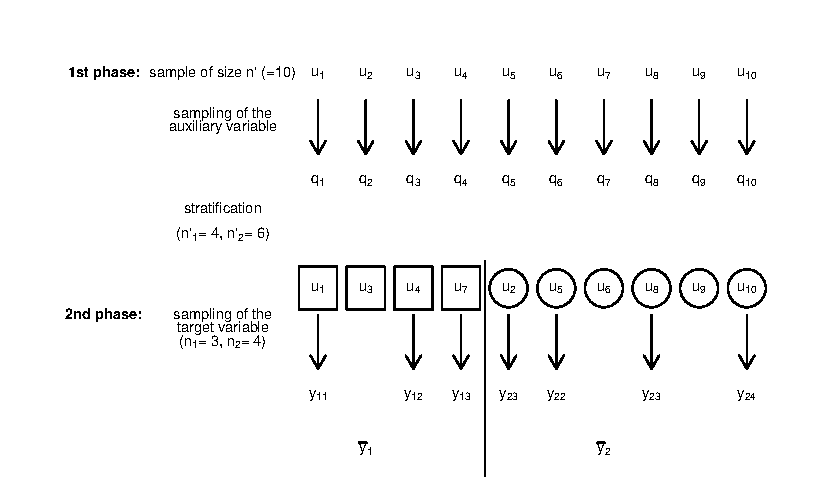
\includegraphics{Grafiken/bm/example.pdf}
\caption{Example 1.}
\label{fig:bm:ex1}
\end{figure}

Further text.

%%%%%%%%%%%%%%%%%%%%%%%%%%%
%% Materials and Methods %%
%%%%%%%%%%%%%%%%%%%%%%%%%%%
\section{Materials and Methods}
\label{sec:bm:methods}

Examples can be found in \citet{Mandallaz_2008} see also \citep{Gregoire_2008,Mandallaz_2008}.

%%-------------------------------------%%
%% Data sampling and sample processing %%
%%-------------------------------------%%
\subsection{Data sampling and sample processing}
\label{subsec:bm:methods:sampling}

\begin{equation}
\widehat{\overline{Y}}_{2st}=\sum^L_{h=1}w_h\frac{1}{n_h}\sum_{i=1}^{n_h}y_{hi}=\sum^L_{h=1}w_h\overline{y}_h
\label{eq:bm:exampleequation1}
\end{equation}

Example Equation \ref{eq:bm:exampleequation1} shows an unbiased estimator.

%%-------------------%%
%% Biomass functions %%
%%-------------------%%
\subsection{Biomass functions}
\label{subsec:bm:methods:bm_functions}

Biomass functions.

%%----------------------%%
%% Sensitivity analysis %%
%%----------------------%%
\subsection{Sensitivity analysis}
\label{subsec:bm:methods:sensitivity}

Sensitivity.

%%-------------------%%
%% Nutrient contents %%
%%-------------------%%
\subsection{Nutrient contents}
\label{subsec:bm:methods:nutrients}

Sensitivity.

%%%%%%%%%%%%%
%% Results %%
%%%%%%%%%%%%%
\section{Results}
\label{sec:bm:results}

%%-------------------%%
%% Biomass functions %%
%%-------------------%%
\subsection{Biomass functions}
\label{subsec:bm:results:bm_functions}

Biomass functions.

%%----------------------%%
%% Sensitivity analysis %%
%%----------------------%%
\subsection{Sensitivity analysis}
\label{subsec:bm:results:sensitivity}

Sensitivity.

%%-------------------%%
%% Nutrient contents %%
%%-------------------%%
\subsection{Nutrient contents}
\label{subsec:bm:results:nutrients}

Nutrient.

%%%%%%%%%%%%%%%%
%% Discussion %%
%%%%%%%%%%%%%%%%
\section{Discussion}
\label{sec:bm:discussion}

%%-------------------%%
%% Biomass functions %%
%%-------------------%%
\subsection{Biomass functions}
\label{subsec:bm:discussion:bm_functions}

Biomass functions.

%%----------------------%%
%% Sensitivity analysis %%
%%----------------------%%
\subsection{Sensitivity analysis}
\label{subsec:bm:discussion:sensitivity}

Sensitivity.

%%-------------------%%
%% Nutrient contents %%
%%-------------------%%
\subsection{Nutrient contents}
\label{subsec:bm:discussion:nutrients}

Nutrients.

%%%%%%%%%%%%%%%%%
%% Conclusions %%
%%%%%%%%%%%%%%%%%
\section{Conclusions}
\label{sec:bm:conclusions}

Conclusion

%%%%%%%%%%%%%%%%%%%%%%
%% Acknowledgements %%
%%%%%%%%%%%%%%%%%%%%%%
\section*{Acknowledgements}
\label{sec:bm:acknowledgements}
We would like to thank the German Science Foundation (DFG) for financial support of this study (Sachbeihilfe SA 415/5-1) and Dr. B�ckmann of the Lower Saxony Forest Planning Office for his kind provision of the inventory data.
Moreover, we would like to thank two anonymous reviewers for their helpful comments.
